
\begin{titlepage}
\begin{center}

% Upper part of the page. The '~' is needed because \\
% only works if a paragraph has started.

\textsc{\large Manual treeCensusODK}\\
\vspace{3cm}
% Title
\HRule \\
{\Large \bfseries Aplicativo de coleta de dados em campo por dispositivo móvel\\}

\HRule 

\vspace{5cm}
\begin{center}
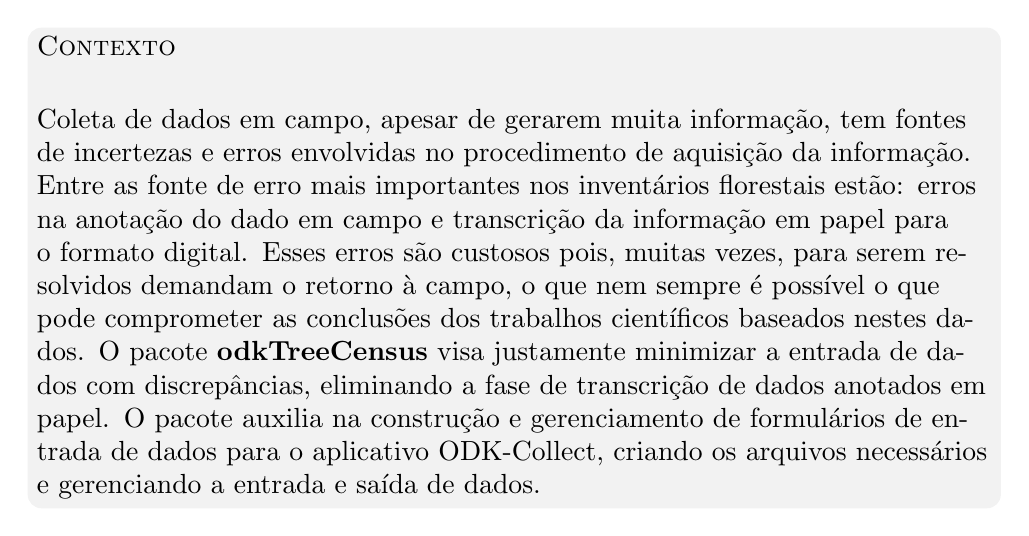
\begin{tikzpicture}
  \node[fill=gray!10!white,rounded corners=5pt,text width=1\textwidth] {
    \textsc{Contexto}\par

    \vspace{.5cm}
Coleta de dados em campo, apesar de gerarem muita informação, tem fontes de incertezas e erros envolvidas no procedimento de aquisição da informação. Entre as fonte de erro mais importantes nos inventários florestais estão: erros na anotação do dado em campo e transcrição da informação em papel para o formato digital. Esses erros são custosos pois, muitas vezes, para serem resolvidos demandam o retorno à campo, o que nem sempre é possível o que pode comprometer as conclusões dos trabalhos científicos baseados nestes dados. O pacote \textbf{odkTreeCensus} visa justamente minimizar a entrada de dados com discrepâncias, eliminando a fase de transcrição de dados anotados em papel. O pacote auxilia na construção e gerenciamento de formulários de entrada de dados para o aplicativo ODK-Collect, criando os arquivos necessários e gerenciando a entrada e saída de dados.    

};
\end{tikzpicture}
\end{center}


\vspace{1cm}



{
\begin{flushright} 
Autor:
Alexandre Adalardo de \textsc{Oliveira}\\
{Departamento de Ecologia - IBUSP}
%\end{minipage}
%\begin{minipage}{0.5\textwidth}
\end{flushright}
}
% \end{minipage}
%\vspace{2cm}
% Bottom of the page
%\HRule\\[0.1cm]

\includegraphics[width=0.3\textwidth]{media/LogoLabtrop3.png}



%\pagebreak

%\includegraphics[width=0.75\textwidth]{Arquivos/restingaPq.png}

% % Author and supervisor
% %\begin{minipage}{0.7\textwidth}
% {
% \begin{flushright} 
% Proponente:
% Alexandre Adalardo de \textsc{Oliveira}\\
% {Universidade de São Paulo, }{Departamento de Ecologia - IB}
% %\end{minipage}
% %\begin{minipage}{0.5\textwidth}
% \end{flushright}
% }
% % \end{minipage}
% %\vspace{2cm}
% % Bottom of the page
% %\HRule\\[0.1cm]
% 
\includegraphics[width=0.3\textwidth]{LogoLabtrop3.png}


\end{center}
\end{titlepage}
